\documentclass[10pt]{article}
\usepackage{amsmath,amssymb}
\usepackage{fontspec}

\setmainfont{Latin Modern Roman}
\newfontfamily\titre{Inter}[UprightFont=* Bold,BoldFont=* ExtraBold]
\usepackage[a4paper,top=1.1cm,bottom=1.35cm,left=1.4cm,right=1.4cm,headheight=0pt,footskip=0.8cm]{geometry}
\usepackage{graphicx}
\usepackage[most]{tcolorbox}
\usepackage{tikz}
\usepackage{enumitem}
\usepackage{fancyhdr}
\usepackage{eso-pic}
\usepackage{multicol}
\usepackage{lastpage}\usepackage{needspace}

% ---------- couleurs Sigma Cap ----------
\definecolor{ink}{HTML}{14284B}
\definecolor{sky}{HTML}{1F8FD0}
\definecolor{lime}{HTML}{6FA82F}
\definecolor{gold}{HTML}{D99A1E}
\definecolor{rouge}{HTML}{C0392B}
\definecolor{violet}{HTML}{6C3FB5}
\definecolor{fond}{HTML}{F2F5F9}

\setlength{\parindent}{0pt}
\setlength{\parskip}{2pt}
\renewcommand{\arraystretch}{1.15}
\newcommand{\R}{\mathbb{R}}
\newcommand{\N}{\mathbb{N}}
\newcommand{\Z}{\mathbb{Z}}
\newcommand{\Q}{\mathbb{Q}}

% ---------- filigrane ----------
\AddToShipoutPictureBG{%
  \AtPageCenter{\makebox(0,0){\rotatebox{50}{\fontsize{78}{78}\selectfont\bfseries\color{ink!6}SIGMA CAP}}}%
  \AtPageLowerLeft{\put(\LenToUnit{0.5\paperwidth},\LenToUnit{0.28\paperheight}){\makebox(0,0){\rotatebox{50}{\fontsize{30}{30}\selectfont\bfseries\color{sky!8}PROFDEMATHS 2.0}}}}%
  \AtPageUpperLeft{\put(0,\LenToUnit{-0.35cm}){\color{ink}\rule{\paperwidth}{0.35cm}}}%
  \AtPageLowerLeft{\put(0,0){\color{lime}\rule{\paperwidth}{0.18cm}}}%
}

% ---------- pied de page ----------
\pagestyle{fancy}\fancyhf{}
\renewcommand{\headrulewidth}{0pt}
\fancyfoot[L]{\scriptsize\color{ink}\textbf{Sigma Cap} -- Vers la réussite · CEM Kennedy}
\fancyfoot[C]{\scriptsize\color{ink!70}\piedfiche}
\fancyfoot[R]{\scriptsize\color{ink}\textbf{\thepage/\pageref{LastPage}}}

% ---------- puces colorées ----------
\setlist[itemize]{leftmargin=1.1em,itemsep=1pt,topsep=2pt,label={\color{sky}\small$\blacktriangleright$}}
\DeclareRobustCommand{\pucenum}[1]{\tikz[baseline=(n.base)]\node[circle,fill=sky,text=white,inner sep=1.3pt,minimum size=1.15em,font=\footnotesize\bfseries](n){#1};}
\setlist[enumerate,1]{leftmargin=1.6em,itemsep=1pt,topsep=1pt,label={\pucenum{\arabic*}}}
\setlist[enumerate,2]{leftmargin=1.5em,itemsep=1pt,topsep=1pt,label={\color{gold}\bfseries\alph*)}}

% ---------- cadres ----------
\newcounter{exo}
\newtcolorbox{exo}[3][]{enhanced,breakable,colback=white,colframe=#2,boxrule=0.9pt,arc=2.5mm,
  left=7pt,right=7pt,top=5pt,bottom=4pt,before skip=3.5pt,after skip=3pt,
  fonttitle=\bfseries\small,coltitle=white,colbacktitle=#2,
  title={\stepcounter{exo}Exercice \theexo\ \ \textcolor{white!85!#2}{\textbullet}\ \ #3},
  attach boxed title to top left={xshift=8pt,yshift=-2.2mm},
  boxed title style={arc=1.5mm,boxrule=0pt},#1}

\newcommand{\partie}[3]{\needspace{7\baselineskip}\vspace{3pt}%
  \begin{tcolorbox}[enhanced,colback=#1,colframe=#1,arc=1.5mm,boxrule=0pt,left=6pt,right=6pt,top=2.5pt,bottom=2.5pt,before skip=4pt,after skip=3pt]
  {\color{white}\bfseries\large #2}\hfill{\color{white}\small\itshape #3}
  \end{tcolorbox}}

\newcommand{\demo}{\tikz[baseline=-0.6ex]\node[fill=violet,text=white,rounded corners=1.5pt,inner sep=1.6pt,font=\scriptsize\bfseries]{DÉMONSTRATION};}
\newcommand{\etoiles}[1]{{\color{gold}\ifcase#1\or$\star$\or$\star\star$\or$\star\star\star$\fi}}

% bulle avec la photo de M. Thiam
\newcommand{\bulle}[1]{%
  \begin{tcolorbox}[enhanced,colback=gold!9,colframe=gold!80!black,boxrule=0.6pt,arc=3mm,
    left=34pt,right=6pt,top=3pt,bottom=3pt,before skip=4pt,after skip=2pt,fontupper=\small,
    overlay={\node[anchor=west] at ([xshift=2pt]frame.west) {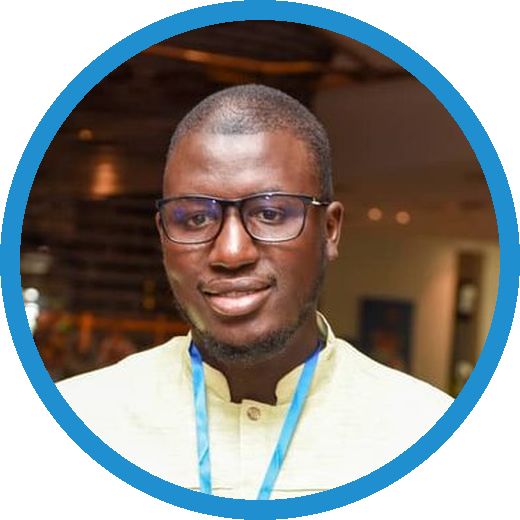
\includegraphics[width=26pt]{thiam-rond.png}};}]
  #1\end{tcolorbox}}

\newcommand{\C}{\mathbb{C}}
\newcommand{\entete}[3]{% titre, chapitre, classe
\vspace*{-2pt}
\begin{tcolorbox}[enhanced,colback=fond,colframe=ink,boxrule=1pt,arc=3mm,left=6pt,right=6pt,top=4pt,bottom=4pt]
\begin{minipage}[c]{0.15\textwidth}\centering\includegraphics[height=2.25cm]{logo-full.jpg}\end{minipage}%
\begin{minipage}[c]{0.70\textwidth}\centering
  {\small\color{sky}\bfseries COURS DE RENFORCEMENT · ANNÉE SCOLAIRE 2026 -- 2027}\\[3pt]
  {\LARGE\color{ink}\bfseries #1}\\[2pt]
  {\large\color{ink}\bfseries #2}\\[4pt]
  \tikz\node[fill=lime,text=white,rounded corners=2pt,inner sep=3pt,font=\small\bfseries]{Classe~: #3};\
  \tikz\node[fill=sky,text=white,rounded corners=2pt,inner sep=3pt,font=\small\bfseries]{Prof~: M. Racine Thiam};\
  \tikz\node[fill=gold,text=white,rounded corners=2pt,inner sep=3pt,font=\small\bfseries]{CEM Kennedy};
\end{minipage}%
\begin{minipage}[c]{0.15\textwidth}\centering\includegraphics[height=2.25cm]{profdemaths.jpg}\end{minipage}
\end{tcolorbox}}
\newenvironment{competences}{%
\begin{tcolorbox}[enhanced,colback=sky!6,colframe=sky,boxrule=0.7pt,arc=2mm,left=6pt,right=6pt,bottom=3pt,
  title={\bfseries\small Compétences travaillées dans cette fiche},fonttitle=\small,colbacktitle=sky,coltitle=white,
  attach boxed title to top left={xshift=8pt,yshift=-2mm},boxed title style={arc=1mm,boxrule=0pt},top=6pt]
\small\begin{multicols}{2}\begin{itemize}}{%
\end{itemize}\end{multicols}\vspace{-6pt}
{\footnotesize\color{ink!80}Niveau~: \etoiles1\ application directe \quad \etoiles2\ entraînement \quad \etoiles3\ approfondissement \qquad \demo\ exercice de raisonnement}
\end{tcolorbox}}
\newcommand{\rappel}[1]{\begin{tcolorbox}[enhanced,colback=lime!7,colframe=lime!70!black,boxrule=0.6pt,arc=2mm,left=6pt,right=6pt,top=3pt,bottom=3pt,before skip=3pt,after skip=3pt,fontupper=\small,title={\bfseries\footnotesize Rappel de cours},colbacktitle=lime!70!black,coltitle=white,attach boxed title to top left={xshift=8pt,yshift=-2mm},boxed title style={arc=1mm,boxrule=0pt},top=5pt]#1\end{tcolorbox}}
